\documentclass{article}

\usepackage{setspace}
\usepackage[utf8]{inputenc}
\usepackage{amsmath}
\usepackage{amssymb}
\usepackage{amsthm}
\usepackage[colorlinks]{hyperref}
\hypersetup{%
    colorlinks=true,
    linkcolor=blue,
    urlcolor=cyan,
    citecolor=blue
}
\usepackage[inline]{enumitem}
\usepackage{mathtools}
\newlist{inlist}{enumerate*}{1}
\setlist[inlist]{label= (\alph*)}
\usepackage{booktabs}
\usepackage{multirow}
\usepackage{graphicx}
\usepackage{smartdiagram}
\usepackage{subcaption}
\usepackage{float}
\floatstyle{boxed}
\restylefloat{figure}
\restylefloat{table}
\usepackage{biblatex}
\addbibresource{sources.bib}
\usepackage[nopostdot,toc,acronym,nomain,nonumberlist]{glossaries}
{\makeglossaries}
\loadglsentries[acronym]{glossary}
\usepackage{tikz}
\usetikzlibrary{shapes,positioning,arrows,calc}

\newcommand{\mylongtitle}{MS Report \\
On the state of formal-verification language technology}
\newcommand{\mysubtitle}{}
\newcommand{\myshorttitle}{}
\newcommand{\mytitle}{\mylongtitle}

% Preamble {{{

% newcommands, DeclareMathOperators, &c. {{{
\theoremstyle{plain} % default
\newtheorem{thm}{Theorem}[section]
\newtheorem{lem}[thm]{Lemma}
\newtheorem{prop}[thm]{Property}
\newtheorem*{cor}{Corollary}

\theoremstyle{definition}
\newtheorem{defn}{Definition}[section]
\newtheorem{example}{Example}[section]
\newtheorem{exercise}{Exercise}[section]
\newtheorem*{prob}{Problem}

\theoremstyle{remark}
\newtheorem*{rem}{Remark}
\newtheorem*{note}{Note}
\newtheorem{case}{Case}

\newcommand{\yields}{\Rightarrow}
\newcommand{\Yields}{\Rightarrow^{\star}}
\newcommand{\union}{\cup}
\newcommand{\intersect}{\cap}
\newcommand{\Union}{\bigcup}
\newcommand{\Intersect}{\bigcap}
\newcommand{\compose}{\mathrel{\circ}}
\newcommand{\comp}[1]{{\overline{#1}}}
\newcommand{\DownTo}{\mathrel{\Downarrow}}
\newcommand{\To}{\mathrel{\Rightarrow}}
\newcommand{\TO}{\mathrel{\Rrightarrow}}
\newcommand{\definedas}{\triangleq}

\newcommand{\bb}[1]{\mathbb{#1}}
\newcommand{\N}{\bb{N}}
\newcommand{\Z}{\bb{Z}}
\newcommand{\Q}{\bb{Q}}
\newcommand{\R}{\bb{R}}
\newcommand{\I}{\bb{I}}

\newcommand{\mc}[1]{\mathcal{#1}}
\newcommand{\Powerset}[1]{\mc{P}\left(#1\right)}

\newcommand{\set}[1]{\left\{#1\right\}}
\newcommand{\setbuild}[2]{\left\{ #1 : #2\right\}}

\newcommand{\var}[1]{\mathit{#1}}
\newcommand{\func}[1]{\mathit{#1}}

\DeclareMathOperator{\false}{false}
\DeclareMathOperator{\true}{true}

\DeclarePairedDelimiter{\abs}{\lvert}{\rvert}
\DeclarePairedDelimiter{\norm}{\lVert}{\rVert}
\DeclarePairedDelimiter{\ceil}{\lceil}{\rceil}
\DeclarePairedDelimiter{\floor}{\lfloor}{\rfloor}

\DeclareMathOperator{\lcm}{lcm}

\newcommand{\idem}{\emph{idem.}}
\newcommand{\vs}{{\emph{v{.}}}}
\newcommand{\ie}{\emph{i.e.}}
\newcommand{\eg}{\emph{e.g.}}
\newcommand{\etc}{\emph{etc.}}
\newcommand{\etal}{\emph{et al.}}

\newcommand{\haltprob}{\emph{Entscheidungsproblem}}
% newcommands, DeclareMathOperators, &c. }}}

% Preamble }}}


\begin{document}

\title{\mytitle}
\author{D. Ben Knoble \\
Department of Computer Science \\
University of North Carolina at Chapel Hill}
\date{April 2020}

\maketitle

\begin{abstract}
    In this report I explore the current state of verified programs research through
several lenses. I begin with a historical background of formal methods before
switching to formal verification in modern programming environments. In
particular, I examine verified user-programs and compilers. Next I categorize
verified programming tools along three (3) axes:
\begin{inlist}
\item interactivity,
\item proof logic, and
\item programming language.
\end{inlist}
Following that, I compare two extended examples of verified programs in
different systems. I also discuss a number of modern research projects and the
impacts they have had on formal verification, especially at scale and in
security-related settings. Lastly, I summarize the challenges of formal
verification in today's settings: notably, these include scaling proofs,
automation and proof management, symbolic explosion, and cross-language
verification. I conclude with a reminder that formal verification is another
tool in the programmer's toolbox and that the programmer must exercise
appropriate judgement in deciding which tool will solve a given problem.

\end{abstract}

Approved by:

Primary reader: Don Porter {\hrulefill}

Secondary reader: Cynthia Sturton {\hrulefill}

\begin{singlespace}
    \newpage
    \tableofcontents

    \newpage
    \listoffigures
    \listoftables
\end{singlespace}

\newpage

\glsresetall[acronym]

\section{Introduction}

First, I introduce the ideas of formal methods and formal verification, in
particular their connection to programming. Next, I briefly dissect the various
layers of abstraction that programmers operate in and the corresponding
layers of verification. Finally, I outline the direction of the rest of the
paper.

\subsection{Background}\label{S:background}

Formal methods are mathematical techniques for describing and verifying system
properties~\cite{Wing_90}. They have been successfully applied to the practice
of programming and computation since the birth of computing:
\citeauthor{Turing_1937}'s famous 1937 discussion of the {\haltprob} is an
application of mathematical reasoning to a generalized system of
computation~\cite{Turing_1937}. The use of formal methods continued throughout
the modern computing era, with \citeauthor{McCarthy_67} formalizing the first
proof of a verified compiler in 1967~\cite{McCarthy_67}. The proof was later
mechanically verified to be correct in 1972~\cite{Milner_72}. The computing
giant and prolific writer \citeauthor{EWD:EWD1036} argued in 1988 that the very
nature of programming depended on notions of symbolic manipulation, formal
semantics, and the task of giving a ``formal proof'' that the proposed program
``meets the equally formal functional specification''---and that Computer
Science education at the time generally omitted much of the relevant background
and material necessary for accomplishing this task~\cite{EWD:EWD1036}.

Formal verification, \citeauthor{EWD:EWD1036}'s act of proving that the program
implements its specification, has not died as he predicted through a ``foggy
crystal ball.'' Instead, they have become increasingly powerful, accessible, and
vital, as I aim to elucidate here. Some computer scientists hesitate to make
claims about the termination of a particular program~\cite{Cook_2011}, perhaps
intimidated by \citeauthor{Turing_1937}'s Halting Problem arguments; yet, proofs
of termination, correctness, non-interference, and more are increasingly
necessary and useful to reason about programs. For example, such proofs are now
used to reason about \gls{os}
kernels~\cite{Klein_EHACDEEKNSTW_09,Klein_AEHCDEEKNSTW_10,Klein_AEMSKH_14,Sewell_KH_16,Narayanan_2019,Narayan_2020,Nelson_2017},
safety-critical systems such as avionics~\cite[\S 1]{Leroy-Compcert-CACM},
in-kernel compilers~\cite{186144,258848}, file-systems~\cite{Zou_2019}, and
concurrent systems~\cite{222565,222621}. These are just a few modern examples in
systems-contexts; verification has made its way into everyday programming, with
applications to, \eg, web-scraping, spatial programming, and superoptimization
for bitvector programs~\cite[\S 4]{Torlak_2013}.

In parallel to the growing efforts of formal verification, rising complexity
presents ongoing challenges to the development and correctness of software. This
is unfortunately coupled with the increasing power of verification tools---the
latter is necessary to make verification of the formal amenable. Consequently,
the verification tools also exhibit increasing complexity, with some being
essentially expert systems\footnote{For a glance at the complexity of some
systems, see~\cite{Jung_2015,Jung_2016,Krebbers_2017a,Jung_2018b} and
\figurename~\ref{F:iris_complex}. In fairness, as we'll see, this complexity
arises from distilling a family of complexities to a simpler base, and then
using that to prove Rust's safety~\cite{Jung_2018a}.}. Other systems combine
automation with domain knowledge to create a narrower, more accessible tool. We
will see some examples of this complexity and automation in
Section~\ref{S:examples}.

\subsection{The Verified Programs Stack}\label{S:stack}

To examine the technology behind verified programs, it will be helpful to
understand the layers of abstraction in today's programming environments and the
corresponding verification layers. I present a brief overview of these layers,
with notes on what I will cover in the remainder of the paper and what is out of
scope; where possible, references are provided for further reading.

The general idea is that, in order to fully trust a program implements its
specification, we should like a proof at the source level and proofs that each
of the intervening levels between source and final execution preserve the
validity of the proof; in other words, that the final result can still be said
formally to implement the specification without the work of repeating the proof
at each stage.

The model presented in \figurename~\ref{F:abstraction} generally ignores
distributed systems and newer environments like the cloud; here I am primarily
concerned with a program running on a single machine, though it is possible to
generalize the model. I also ignore containerization, orchestration, and build
and deployment pipelines insofar as they are represented as user-space programs
or compositions thereof. Build pipelines naturally include compilers, which are
shown in the model despite being user-space programs. Much of the technology we
will see in this paper has been or can be extended to these domains.

Also out of scope is full-stack verification in the vein of
IronClad~\cite{hawblitzel2014ironclad} and
IronFleet~\cite{hawblitzel2015ironfleet}. Here I am considering the individual
components, especially the top layers.

\begin{figure}[hb]
    \centering
    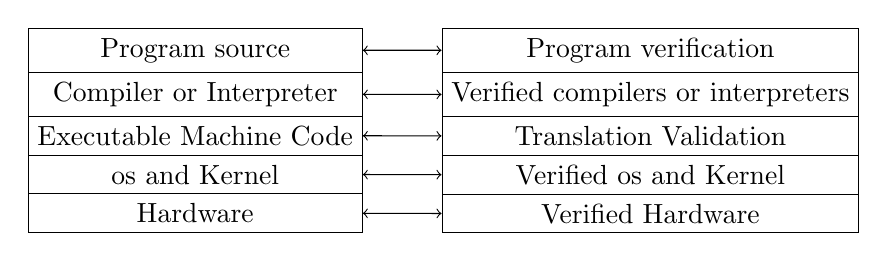
\begin{tikzpicture}[stack/.style={rectangle split, rectangle split parts=5, draw, anchor=center}]
        \node[stack](prog){%
            \nodepart{one}Program source
            \nodepart{two}Compiler or Interpreter
            \nodepart{three}Executable Machine Code
            \nodepart{four}\gls{os} and Kernel
            \nodepart{five}Hardware
        };
        \node[stack,right=of prog](verification){%
            \nodepart{one}Program verification
            \nodepart{two}Verified compilers or interpreters
            \nodepart{three}Translation Validation
            \nodepart{four}Verified \gls{os} and Kernel
            \nodepart{five}Verified Hardware
        };
        \draw[<->] (prog.one east) -- (verification.one west);
        \draw[<->] (prog.two east) -- (verification.two west);
        \draw[<->] (prog.three east) -- (verification.three west);
        \draw[<->] (prog.four east) -- (verification.four west);
        \draw[<->] (prog.five east) -- (verification.five west);
    \end{tikzpicture}
    \caption{A simplified programming environment and execution stack, with corresponding verification technology}\label{F:abstraction}
\end{figure}

At the very top of the stack, we have the program source. Whether high-level or
low-level, this is the definition of what we want the computer to do.
Verification requires a formal specification of that behavior and a proof that
the source-as-written, coupled with the language's formal semantics, implement
that behavior. We will study almost entirely tools and techniques for
accomplishing this task. Some key components include
\begin{inlist}
\item the kind of verifier (\eg, push-button or interactive);
\item the logic of the verifier (\eg, \gls{smt} or higher-order constructive
    propositional logic via \gls{coc}); and
\item the logical system of the proof (\eg, separation logic).
\end{inlist}

In order to execute the program, we have the remaining layers. In order:
\begin{enumerate}
    \item\label{i:stack_translator} A program translator (compiler or
        interpreter)\footnote{These are almost eschewed in the case of the
        assembly programmer; yet, there is still the assembler or linker to
        contend with.}
    \item\label{i:stack_asm} The produced executable machine code (\eg, ELF
        binaries)
    \item\label{i:stack_OS} The \gls{os} and kernel responsible for managing execution
        of the machine code
    \item\label{i:stack_hardware} The underlying hardware that carries out the
        instructions
\end{enumerate}

Items~\ref{i:stack_OS} and~\ref{i:stack_hardware} are out of scope for this
paper. I refer the interested reader to research on verified \gls{os} and
kernels~\cite{Klein_EHACDEEKNSTW_09,Klein_AEHCDEEKNSTW_10,Klein_AEMSKH_14,Sewell_KH_16,Narayanan_2019,Narayan_2020,Nelson_2017}
and on verifying
processors~\cite{sturton-memocode13,Sturton_2013,Bradfield_2016,zhang2017identifying,zhang2018recursive,zhang2018end}.

Item~\ref{i:stack_asm} is particularly interesting and has generated much work
on translation validation~\cite{Pnueli_1998}. This kind of verification proceeds
by validating each run of a compiler, comparing the executable code to the
source and guaranteeing that a \emph{particular} set of executable code
implements a \emph{particular} set of program source code. I will have only
slightly more to say on this subject when we get to verified compilers; I point
the interested reader to works such
as~\cite{Sewell:phd,Sewell_KH_16,Sewell_2013,Necula_2000}.

This leaves item~\ref{i:stack_translator}, the program translator. In
safety-critical systems, it is vital that there be no miscompilation, \ie, bugs
introduced by compilation. Even outside of such restrictive domains, it is
important to trust that the compiler faithfully compiles source code; otherwise,
our systems are all subject to vicious attack~\cite{Thompson_1984}. Thus a
verified compiler\footnote{with verified interpreters a combination of an
on-the-fly compiler and a user-space program, though they have their own unique
challenges} is an important component in the software-development tool-chain.
Verifying a compiler amounts to both a proof about a particular program---the
compiler itself---\emph{and} a proof about a \emph{class} of programs---those
accepted and generated by the compiler. One hopes that a verified compiler
preserves proofs about the source; that is, if a program \(S\) is proven to have
some property \(P\) (written \(S \models P\) after~\cite{Leroy-Compcert-CACM}),
compiling with a verified compiler \(C\) should imply that \(C(S) \models P\).
Thus we have a statement about an entire class of programs, and it is this type
of statement that allows the composition of proven layers to itself be proven.

\subsection{Structure of this report}

In Section~\ref{S:categories} I propose to classify the tools used to verify
programs. In Section~\ref{S:examples} I look at a few examples of verified
programs and identify a few prominent strategies and challenges. In
Section~\ref{S:discussion} I discuss the frontier of the formal-methods and
verified programs research, attempting to answer the question ``What are the
next big challenges to tackle for program verification?'' Finally, I conclude
with Section~\ref{S:conclusion}.


\section{Categorizing Verified Programming Tools}\label{S:categories}

I propose 3 axes along which to classify the tools used to verify programs.
These are
\begin{enumerate}
    \item the type of interaction;
    \item the type of proof logic; and
    \item the type of programming languages.
\end{enumerate}

I examine each in turn in Sections~\ref{S:t_interaction},~\ref{S:t_logic},
and~\ref{S:t_pl}.

One might also include the logic of the underlying verifier, especially in cases
where it differs from the proof logic. I choose not to include the verifier's
logic because in the cases I have studied they are the same (\eg, a Coq program
proven in Coq~\cite{Coq}), one is encoded in the other (\eg, a
Dafny~\cite{leino2010dafny} program proven by translation to
Boogie~\cite{Barnett_2006,leino2008this}), or one is not relevant to the other
(\eg, proofs in Iris's logic~\cite{Jung_2018b} use Iris's proof rules, yet
Iris is built on Coq). The encapsulation provided by many verifiers obviates a
need to consider their underlying logics. Except in the case of a leaky
abstraction~\cite{Spolsky_2002}, wherein the underlying verifier's logic leaks
out to the logic of the proof, the programmer tasked with writing the proof is
concerned with the proof logic and the proof to be written. The
programmer interested in building a programming language for verified languages
should certainly study verification logic, in addition to verification logics
like \gls{smt} or \gls{coc} and the architectures of such verifiers (\eg, for
\gls{smt}, the original~\cite{Davis_1960,Davis_1962} or the newer
handbook~\cite{biere2009handbook}).

\subsection{Type of Interaction}\label{S:t_interaction}

In the context of a verified programming tool, ``interaction'' means that
between the programmer and the verifier: what is necessary to formulate proofs?
Borrowing the terminology of~\cite[\S 2]{Nelson_2019}, I dissect this axis into
3 major types of interaction.
\begin{description}
    \item[Interactive tools.] The programmer manually constructs the proof by
        manipulating facets of the tool, such as by invoking tactics, to
        progress towards a specified proof goal. Such tools may provide
        automation or proof-search mechanisms.
    \item[Auto-active tools.] The programmer and the tool share the burden of
        constructing a proof: the tool is capable of some automatic reasoning,
        but requires the programmer to manually fill in the gaps.
    \item[Automatic tools.] Sometimes called ``push-button'' tools. The
        programmer invokes the tool, which might find a proof, fail to find a
        proof, or produce a counter-example.
\end{description}

For each type, see \citeauthor{Nelson_2019}~\cite{Nelson_2019} for further
examples.

\subsubsection{Interactive verification}

This is the model employed by interactive theorem-provers and proof-assistants
such as Coq~\cite{Coq}, Isabelle~\cite{Isabelle}, and HOL~\cite{HOL}. The
programmer, having written programs and specifications, states theorems relating
them (or lemmata, corollaries, \etc, as the case may be). In order to prove the
statements, the programmer interacts directly with the verifier in a sort of
call-and-response. The verifier presents a goal: prove this statement. The
programmer can execute tactics to manipulate the goal, introduce quantified
variables and hypotheses, and otherwise make progress towards the proof of the
goal. The verifier represents the effect of these executions with another
response, \eg, prove this statement in this context. The programmer continues
this dialogue with the verifier, perhaps walking backwards and trying a
different approach or walking forwards through the steps of the proof, until the
verifier has been given a complete proof of all necessary goals.

\begin{figure}[ht]
\begin{coq_example}
Goal forall P: Prop, P -> P.
intros.
assumption.
Qed.
\end{coq_example}
    \caption{Proving a simple tautology in Coq.}\label{F:coq1}
\end{figure}

The example in \figurename~\ref{F:coq1} demonstrates one Coq proof of a
simple tautology through tactics. The \texttt{intros} tactic introduces
quantified variables for manipulation; \texttt{assumption} looks for a
hypothesis in the context that matches the goal.

Such verifiers may support automation in the sense of tactics that invoke other
tactics based on the goal or context; these can range from proof searches to
constraint solvers over linear integer arithmetic to manipulations necessary to
hide details of the underlying logical verifier.

\begin{figure}[ht]
\begin{coq_eval}
Require Import List.
Import ListNotations.
\end{coq_eval}
\begin{coq_example}
Goal In 5 [1;2;3;4;5].
simpl; right; right; right; right.
(* too manual, try again *) Undo.
repeat (try (left; reflexivity); right).
Qed.
\end{coq_example}
    \caption{Proving a tedious proof with automation in Coq.}\label{F:coq2}
\end{figure}

For example, the proof in \figurename~\ref{F:coq1} is completely finished by
tactics like \texttt{tauto} or \texttt{auto}. Advanced automation can be used to
show \(5 \in [1,2,3,4,5]\), where the \(\func{In}\) relation below is computed
as follows: \(\func{In}\) is false for any value and the empty list.
\(\func{In}\) is true if either the value is the head of the list or it is in
the tail of the list. Without automation, the proof consists of the
\texttt{right} tactic four times to get to the correct disjunct; only then can
we finish by selecting the \texttt{left} case and proving it (trivially, \(5 =
5\)). This is explicated in \figurename~\ref{F:coq2}.

\subsubsection{Auto-active verification}

\begin{figure}[ht]
    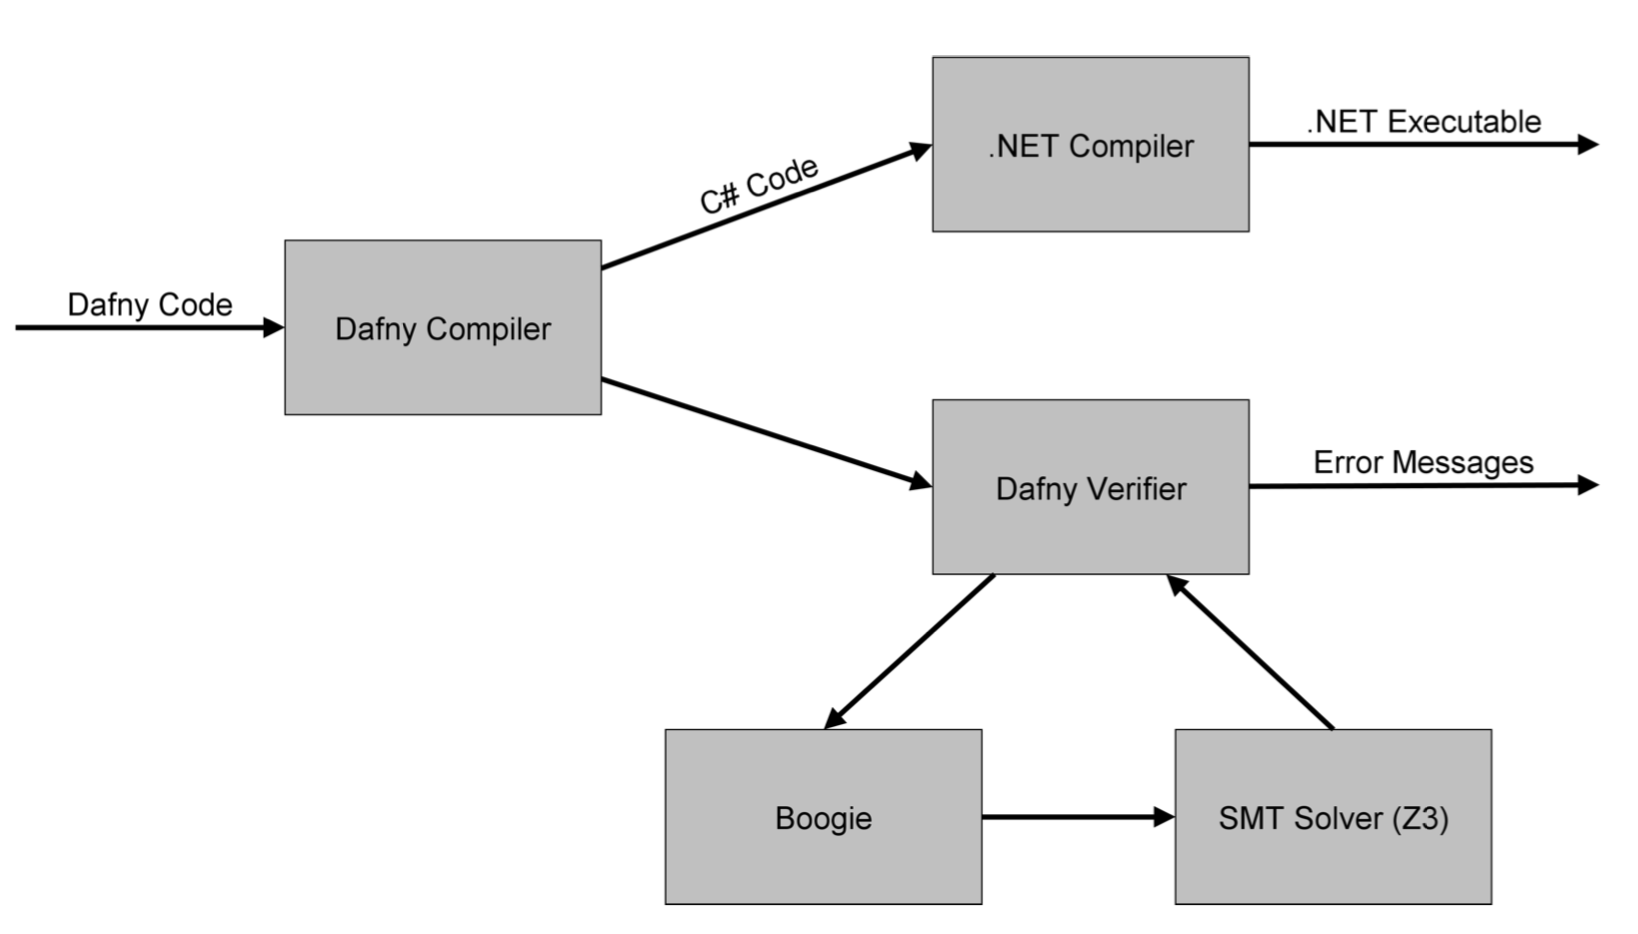
\includegraphics[width=\textwidth]{img/dafny_architecture}
    \caption{Dafny compilation and verification
    architecture~\cite{Herbert2012}}\label{F:dafny_arch}
\end{figure}

The approach taken by verifiers like Dafny~\cite{leino2010dafny}. The programmer
annotates code both with specifications and proof hints, such as pre- or post-
conditions or loop invariants. The verifier translates the source into a
verification condition and uses a constraint solver to finish the verification.
\figurename~\ref{F:dafny_arch} provides an overview of this architecture. Some
verifiers, such as Dafny, permit annotations that nearly rise to the level of
proof texts like those of interactive verification, with composable theorems and
lemmata in addition to functional specifications and standard annotations. While
writing the proofs, though, the current state of the  goal and proof context are
often hidden or implicit, since the verifier translates the goal and context for
the constraint solver\footnote{The original goal and context are of course
visible in the original statement being proven.}. A call-and-response effort is
possible in such verifiers to complete a proof, but a major challenge is to
discover what the automatic part of the verifier cannot prove and actively
provide effective hints to make progress. One power of this type of verifier is
to free the programmer from all the details of the proof; the verifier often can
handle simple statements on its own, and more complex statements can be proven
with only a few well-directed hints. On the other hand, discovering which hints
to use is like a game of ``20 Questions''\footnote{The programmer asks ``Would
you be able to make progress on the proof if I could convince you of \(P\)?''
Based on the verifier's response, which is essentially ``yes'' or ``no'', a
sub-proof of \(P\) is given through hints or not, and the game continues. The
summer course in~\cite{Kapritsos_2020} provides a detailed look at this style of
proof in Dafny.}, and the resulting proofs can be difficult to read.

\begin{figure}[ht]
\begin{verbatim}
predicate IsPrime(i:nat)
{
  i > 1 && (forall j | 1 < j < i :: i % j != 0)
}

method Main() {
  assert forall P :: P ==> P;
  assert 5 in [1,2,3,4,5];
  assert !IsPrime(0);
  assert !IsPrime(1);
  assert IsPrime(2);
  assert IsPrime(3);
  // counter example for the proof to work
  assert 6 % 3 == 0;
  assert !IsPrime(6);
}
\end{verbatim}
    \caption{Example auto-active proofs in Dafny. Responses are provided upon
    invoking the Dafny compiler.}\label{F:dafny_ex}
\end{figure}

The example proofs (\(\forall P: P \implies P\) and \(5\) is in a long list
containing \(5\)) in Dafny are completely automatically checked by the Dafny
compiler, as shown in \figurename~\ref{F:dafny_ex}. However, let's add the
\(\func{IsPrime}\) predicate. Dafny can automatically find proofs for the
primality of 0, 1, 2, and 3. At 6, however, Dafny doesn't know what to do, and
the hint \(6 \mod 3 = 0\) is necessary to prove 6 is not prime. Removing the
line causes a verification error; adding it gives Dafny enough to disprove the
disjunct. Discovering that this is the missing information is rather like taking
an educated guess.

\subsubsection{Automatic verification}

The approach taken by Rosette~\cite{Torlak_2013}. An automatic verifier
restricts the class of properties and programs that be verified in order to
fully automate the process. The essential limit is finitization: finite
specifications that can be implemented without unbounded loops allows symbolic
evaluation or execution to generate constraints that can be handed off to a
solver, much like in auto-active verification. The developer thus programs in
such a restricted verifier and pushes the ``verify button'', invoking the symbolic
evaluator and constraint solver. The limitations allow a greater degree of
automation than in the previous cases, leading to the descriptor ``push-button
verification''---no proof annotations are necessary. Such verifiers have been used
to build surprisingly sophisticated programs given the finitization requirement;
examples include the Yggdrasil file-system~\cite{Sigurbjarnarson_2016} and the
Hyperkernel \gls{os}~\cite{Nelson_2017}.

\begin{figure}[ht]
\begin{verbatim}
#lang rosette

;; Let x be any integer
(define-symbolic x integer?)

;; Let b be any bool
(define-symbolic b boolean?)

;; Verify that b => b for any boolean b
(verify (assert (=> b b)))

;; Verify that |x| >= 0 for any integer x
(define (abs x) (if (>= x 0) x (- x)))
(verify (assert (>= (abs x) 0)))

(verify (assert (member 5 '(1 2 3 4 5))))

(define (prime? n)
  (and (> n 1)
       (andmap (compose1 not zero? (curry modulo n))
               (build-list (- n 2) (curry + 2)))))

(verify (assert (not (prime? 0))))
(verify (assert (not (prime? 1))))
(verify (assert (prime? 2)))
(verify (assert (not (prime? 6))))
\end{verbatim}
    \caption{Example automatic proofs in Rosette. Running the program with
    Racket shows that the assertions are verified.}\label{F:rosette}
\end{figure}

\figurename~\ref{F:rosette} demonstrates the same proofs from before, and a
proof that \(\forall x: \abs{x} \ge 0\), all of which are accomplished
completely automatically by Rosette. In particular, the primality and membership
proofs use Rosette's partial evaluation, so that the statements are effectively
proving a constant truth value.

A related challenge is exponential path explosion: symbolic evaluation may have
to consider a rapidly growing number of symbolic paths while generating
constraints. Rosette takes steps to solve this via aggressive partial
evaluation~\cite{Torlak_2013,Torlak_2014}, lenient symbolic
execution~\cite{Chang_2018}, and
profiling~\cite{Bornholt_2018,Porncharoenwase_2020}. Also related, as in the
case of auto-active verification, is the challenge of communicating back to the
developer the meaning of the results in the program domain.

\subsection{Type of Proof Logic}\label{S:t_logic}

\begin{figure}[ht]
    \centering
    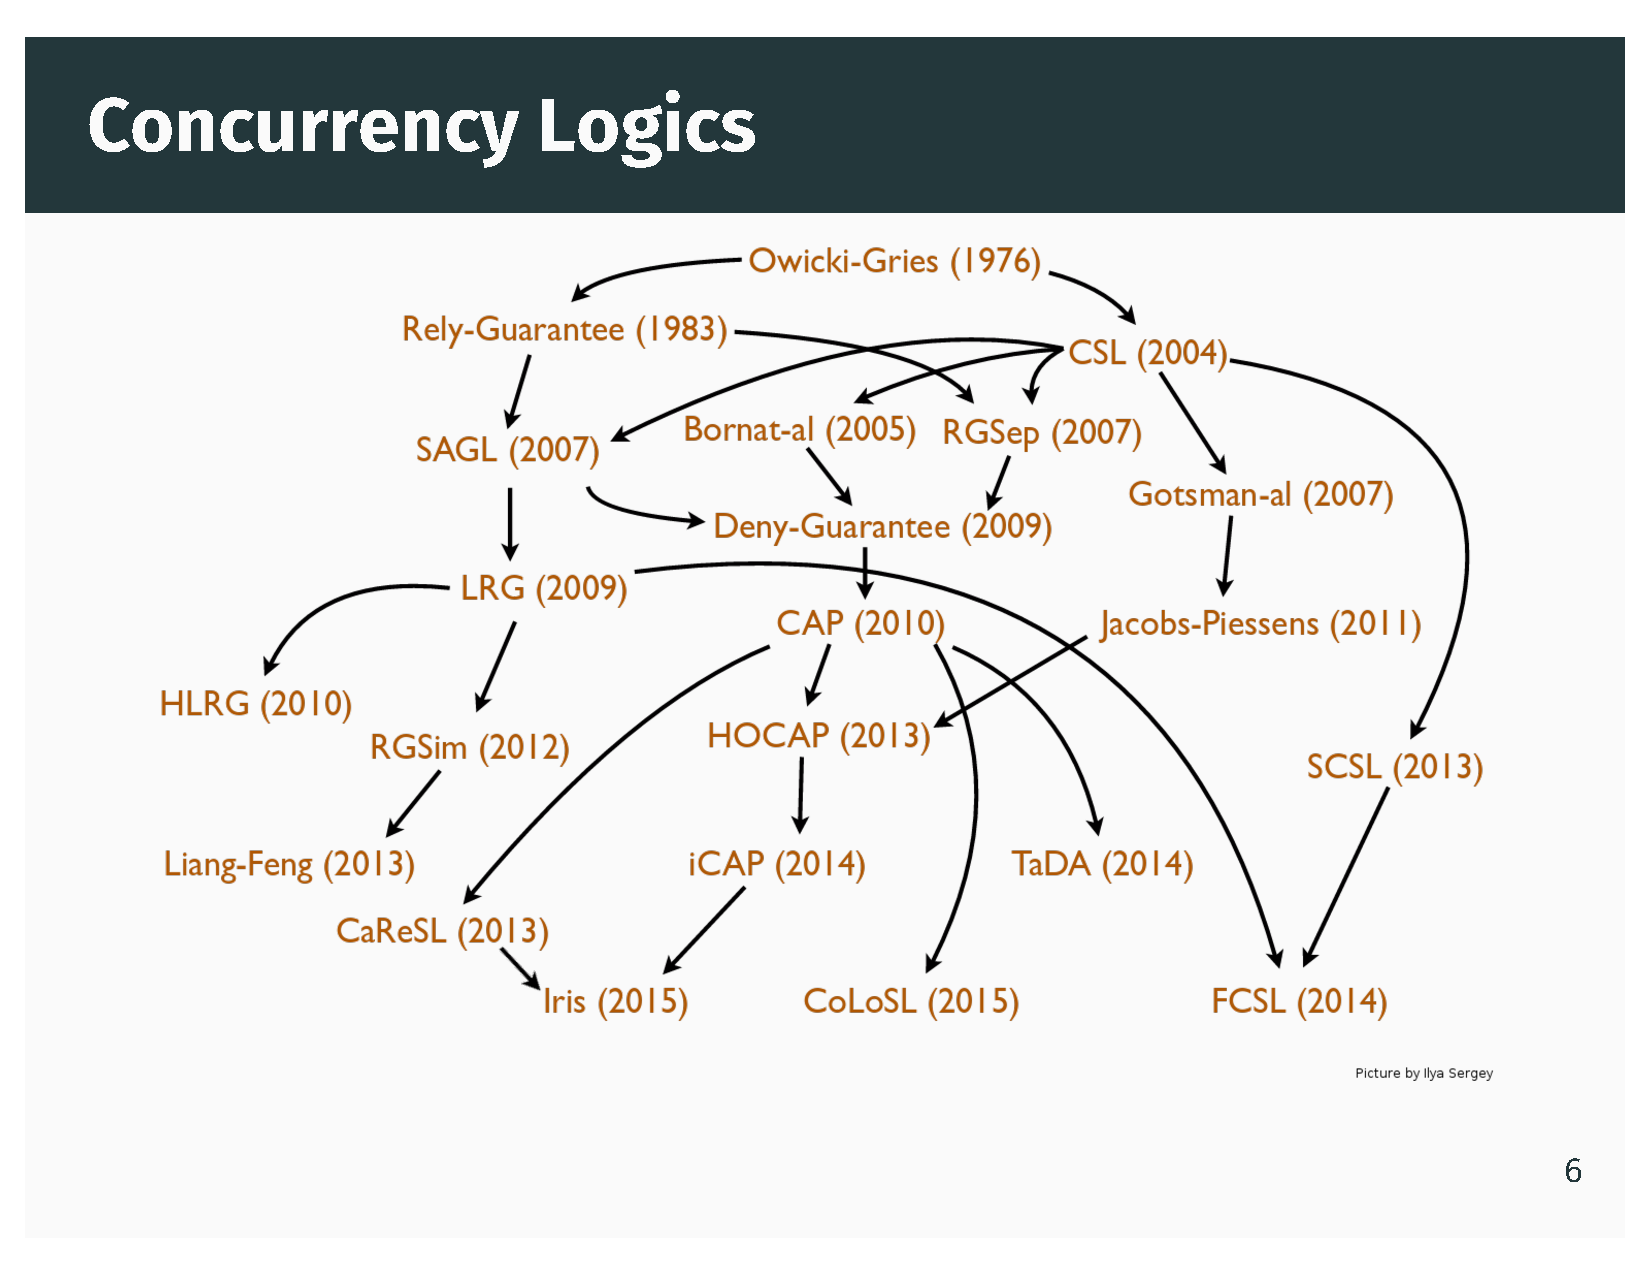
\includegraphics[width=\textwidth]{img/iris_2_0_concurrent_logics}
    \caption{A figure from a presentation on Iris~\cite{Jung_2016_slides}
    depicting the relationship of many concurrent separation logics developed
    specially for a system or proof. Iris notably attempts to distill these
    logics to their core, providing a verifier inside of which any of the
    individual logics may be derived.}\label{F:iris_complex}
\end{figure}

A full account of proof logics for programs would be a long paper in its own
right and is out of scope for this report. Look no further than
\figurename~\ref{F:iris_complex} to see how complicated the topology of (a
subset of) proof logics can be. Instead, I will mention a key proof logic
(namely, Hoare logic) and some of its extensions. For another explanation of
program and proof logics and their uses, see~\cite[\S 5]{Appel_2011}.

\begin{figure}[ht]
    \centering
    \begin{mathpar}

        \inference[\iname{E-APlus}]{%
            \eval{\(e_1\)}{\sigma} = n_1 &
            \eval{\(e_2\)}{\sigma} = n_2
        }{\eval{\(e_1\) + \(e_2\)}{\sigma} = n_1 + n_2}

        \and

        \inference[\iname{E-Seq}]{%
            \comp{\(c_1\)}{\sigma_1} \DownTo \sigma_2 &
            \comp{\(c_2\)}{\sigma_2} \DownTo \sigma_3 &
        }{\comp{\(c_1\);\(c_2\)}{\sigma_1} \DownTo \sigma_3}

    \end{mathpar}
    \caption{Sample inference rules for \texttt{Imp}, a simple imperative
    language. \iname{E-APlus} shows how to add two arithmetic expressions.
    Similarly, \iname{E-Seq} shows how to sequence two statements \(c_1,
    c_2\).}\label{F:Imp_ex}
\end{figure}

All proof logics for programs combine a set of logic rules with the semantics of
the program's language. In the simplest case, the programmer combines
``regular'' logic (in the sense of \gls{coc} or ZFC) with the semantics to write
proofs about program equivalences, termination, and transformations.
\emph{Software Foundations} provides an introduction to proving interesting
meta-theoretic\footnote{``meta'' because they are ``properties of the language
as a whole, rather than of particular programs''~\cite{Pierce:SF2}. It is also
possible to prove claims about specific programs this way, but, at least in some
verifiers, this becomes unwieldy.} claims about a language using these
techniques in Chapters \emph{Simple Imperative Programs}~\cite{Pierce:SF1} and
\emph{Program Equivalence}~\cite{Pierce:SF2}. Essentially, standard reasoning
rules about logic formulae are combined with the inference rules that define the
semantics. An example is provided in \figurename~\ref{F:Imp_ex}. We use the
following notation:

\begin{itemize}
    \item \(\eval{e}{\sigma} = x\) means ``evaluation of \(e\) under a state
        \(\sigma\) produces \(x\)'', and

    \item \(\comp{c}{\sigma} \DownTo \sigma'\) means ``computing statement \(c\)
        in state \(\sigma\) produces the new state \(\sigma'\).''
\end{itemize}

We refer the reader to~\cite{Winskel_1993,Harper_2016} for introductions to
program semantics.

\subsubsection{Hoare Logic}

When turning to program verification\footnote{Recall \citeauthor{EWD:EWD1036}'s
act of proving a program implements its specification.}, \emph{Software
Foundations} introduces Hoare logic. Hoare logic, with its many variations, is
the predominant proof logic for program verification. Originating in
\citeyear{Hoare_1969}~\cite{Hoare_1969}, Hoare logic formalizes the notion of
pre- and post-conditions with the \emph{Hoare triple}, written

\begin{equation*}
    \{P\} C \{Q\},
\end{equation*}

to indicate that command \(C\) has pre-condition \(P\) and post-condition \(Q\),
both assertions. As an example, consider
the pre-condition \(X = 1\) and the command \(X \gets X + 1\) with the obvious
semantics. It is easy to prove the post-condition \(X = 2\). We call such
conditions \emph{assertions}---they map a state \(\sigma\) to a claim about the
state, such as ``In state \(\sigma\), \(X\) is 1.''

The triple states that, if \(P\) is established, executing \(C\) establishes
\(Q\) (or \(C\) does not terminate). This statement can thus be written using
notation from \figurename~\ref{F:Imp_ex}, with \(P\) and \(Q\) assertions about
the state of the program. We write \(\definedas\) to indicate a definition.

\begin{align*}
    \{P\} C \{Q\} \definedas \forall \sigma_1, \sigma_2 &: \comp{c}\sigma_1 \DownTo \sigma_2 &\text{if \(\mathtt{c}\) terminates} \\
    &\implies P\, \sigma_1 &\text{and if \(P\, \sigma_1\) holds} \\
    &\implies Q\, \sigma_2 &\text{then we can establish \(Q\, \sigma_2\) holds.}
\end{align*}

The programmer indicates that \(C\) does not terminate, or that \(C\)
\emph{diverges}, in a Hoare triple by choosing \(Q = \bot\). Since termination
is a hypothesis in the Hoare triple, showing \(C\) does not terminate leads to a
contradiction, from which we can derive \(\bot\). Hoare logic permits reasoning
about partial correctness; termination must be proven
separately\footnote{Various sources claim it is possible to give rules for total
correctness; the most complete rule I have seen involves bounding loops with a
well-founded order.}.

This is a model-theoretic Hoare logic: the proof rules are stated in terms of
the model. Hoare logic can also be defined in proof theory; this is arguably
more common~\cite[Ch.\ \emph{Hoare Logic as a Logic}]{Pierce:SF2}.
Proof-theoretic Hoare logic avoids ascribing direct meaning to Hoare triples and
instead gives syntactic derivation rules. The proof-theoretic derivation rules
are the same judgements as in the model-theoretic definition, and the two are
consistent with each other.

\begin{figure}[ht]
    \centering
    \begin{mathpar}

        \inference[\iname{Hoare-Consequence-Pre}]{%
            \{P'\} C \{Q\} & P \TO P'
        }{\{P\} C \{Q\}}

        \and

        \inference[\iname{Hoare-Seq}]{%
            \{P\} C_1 \{Q\} & \{Q\} C_2 \{R\}
        }{\{P\} C_1;C_2 \{R\}}

    \end{mathpar}
    \caption{Two examples of the rules of Hoare logic.
    \iname{Hoare-Consequence-Pre} captures the notion that we can strengthen the
    pre-condition from \(P'\) to \(P\) and still have a valid triple.
    \iname{Hoare-Seq} provides an analogue to \iname{E-Seq} from
    \figurename~\ref{F:Imp_ex}. The programmer composes rules like these rather
    than invoking the definition of a Hoare triple whenever possible, using a
    higher level of abstraction.}\label{F:Hoare_ex}
\end{figure}

Reasoning with Hoare logic mimics the structure of the program, as triples can
be effectively combined to build up claims about the entire program. The rules
for doing so resemble those of ``regular'' logic formulae above, with theorems
for strengthening pre-conditions or weakening post-conditions. Formalizations
and uses of these rules often work backwards; the natural way to construct a
Hoare logic proof is to start at the final post-condition and move backwards to
the beginning. A selection of rules are presented in
\figurename~\ref{F:Hoare_ex}. We introduce the notation \(P \TO P'\), which is
analogous to implication: the definition is \(\forall \sigma: P\, \sigma
\implies P'\, \sigma\).

I should note that, although Hoare logics are mostly seen for imperative
programming languages, they are also applicable to functional languages. For
example, Iris~\cite[\S 5.1]{Krebbers_2017b} and the RustBelt project~\cite[\S
3.2, esp. \figurename~3]{Jung_2018a} have demonstrated the applicability of a
particular kind of Hoare logic to both \(\lambda\)-calculus style and ML-like
languages.

\subsubsection{Pre-, post-, and weakest conditions}

The choice of pre- and post- conditions is up to the programmer, who wants to
prove that the program implements a specification \(\var{Spec}\). A natural
choice for the post-condition is some \(Q\) that implies \(\var{Spec}\).
Similarly, a natural choice for the pre-condition is some \(P\), possibly
corresponding to constraints on the program inputs, and that also allows the
programmer to prove \(\{P\} C \{Q\}\). Then we can claim that if \(C\)
terminates under pre-conditions \(P\) then \(P \implies C \models \var{Spec}\).

The programmer could also choose \(P = \bot\), in which case any post-condition
at all is valid, including the \(Q\) that entails \(\var{Spec}\) from earlier
(check the definition of the triple, and observe that this is a case of the
principle of explosion). But this ridiculous pre-condition is never satisfied,
so in practice we have proven nothing about \(C\), except that if it terminates
any behavior whatsoever is allowed!

In a similar vein, we can always add extraneous information to the pre-condition
which is not used; this does not necessarily invalidate our proof in the same
way, but such information may not be needed. It is convenient to avoid
unnecessarily strengthening pre-conditions in the overall program statement, as
they might unnecessarily restrict the proof's application to the program. An
example will clarify: consider \(\{X = 1\}X \gets X + 1\{X > 0\}\) with \(X \in
\Z\) and the command \(X \gets n\) indicating assignment of \(n\) to \(X\).
Clearly, the precondition is sufficient to establish the post-condition, but
proving this triple only establishes the program's correctness when \(X = 1\).
If we are interested in more than this narrow situation, we need a weaker
pre-condition; otherwise, we are constrained to only trusting the program when
\(X = 1\) holds. In this particular case, we only need to know that \(X + 1 >
0\), \ie, \(X \ge 0\). Now our program is provably correct in many more cases.

To prevent such absurd pre-conditions as \(\bot\) and to streamline their
generation, many verifiers make use of ``weakest
pre-conditions''~\cite{dijkstra1976discipline,Nelson_1989} (cited
in~\cite{leino2008specification}). The intuitive idea is that for some statement
\(C\) and some post-condition \(Q\) we denote by \(\wpre{C, Q}\) the ``minimal''
non-\(\bot\) information we need to correctly establish \(Q\), \ie, such that
the triple \(\{\wpre{C,Q}\} C \{Q\}\) is provable and the pre-condition is not
\(\bot\). Formally, \(P\) is a weakest pre-condition with respect to \(C\) and
\(Q\) (\(P = \wpre{C,Q}\)) iff \(\{P\} C \{Q\}\) and \(\forall P': \{P'\} C
\{Q\} \implies (P' \TO P)\).

The function \(\func{wp}\) is computable by structural induction on
\(C\). Crucially, it is not a decidability function; it returns a proposition,
not a proof. An extended example is found in~\cite[\S 3]{leino2008specification},
where weakest pre-conditions provide the vehicle used to translate from
Dafny~\cite{leino2010dafny} to Boogie~\cite{Barnett_2006,leino2008this}.

The programmer must still choose an appropriate \(Q\) to establish
\(\var{Spec}\); the generation of the required pre-conditions can be automated
by use of \(\wpre{\cdot,Q}\). Note that this does not mean the proof will be
straightforward with \emph{only} these pre-conditions. The programmer may need
to make logical leaps to strengthen conditions as necessary, particularly where
complex algebraic reasoning is required.

\subsubsection{Separation Logic}

According to~\cite[\S 5]{Appel_2011}, ``Ordinary Hoare logics have difficulty
with pointers and arrays, especially with updates of fields and array slots.''
To solve this problem, \citeauthor{Reynolds} invented \emph{separation
logic}~\cite{Reynolds}.

The crucial extension is to differentiate between the assertion \(P \land Q\),
which denotes that both conjuncts hold on the current state, and the assertion
\(P * Q\), which denotes that each conjunct holds on a disjoint part of the
current state. In other words, the state \(s\) can be split into \(\sigma_1,
\sigma_2\) (often written \(\sigma = \sigma_1 \uplus \sigma_2\)) such that \(P\)
holds on \(\sigma_1\) and \(Q\) holds on \(\sigma_2\). Along with rules for
manipulating this new separating conjunction, the programmer gains the ability
to reason about separate parts of the store or state. Other important rules in
separation logics correspond to framing the state needed by execution of the
program and address- and pointer- manipulation. Together, these rules facilitate
reasoning about pointers and data-structures. The separation of state also
facilitates local reasoning---the correctness of a part of the program is
allowed to depend only on the part of the state it uses. Once that part of the
program is proven correct, we can separately extend the used state with unused
state via the frame rule. The extension does not affect correctness and
guarantees that the unused part of the extended state is not modified by the
program. \figurename~\ref{F:frame} demonstrates the frame rule; notice the side
condition that none of the variables modified by \(C\) are free in \(R\).

\begin{figure}[ht]
    \centering
    \begin{mathpar}
        \inference[\iname{Frame}]{%
            \{P\} C \{Q\} & \func{mod}(C) \intersect \func{fv}(R) = \emptyset
        }{\{P * R\} C \{Q * R\}}

        \and
    \end{mathpar}
    \caption{The frame rule from separation logic which allows extension of the
    proof with disjoint state.}\label{F:frame}
\end{figure}

\subsubsection{Concurrent Separation Logic}

For reasoning about concurrency, Hoare logic and separation logic remained
inadequate; \citeauthor{O_Hearn_2007} proposed a \emph{concurrent separation
logic} to solve the problem~\cite{O_Hearn_2007}. \citeauthor{Brookes_2007}
provides a model in the companion paper~\cite{Brookes_2007}. Both papers discuss
the difficulty of ensuring that such a logic is \emph{sound}, \ie, that every
provable formula in the logic is semantically valid. The soundness problem
coupled with the plethora of available separation and concurrent logics
(\figurename~\ref{F:iris_complex}), each with their own complex rules,
demonstrate the difficulty both of developing and reasoning in a concurrent
separation logic. Reasoning about parallel programs may bring inherent
complexity to the problem. The various concurrent logics add rules required for
their specific uses, \eg, partial ownership or permissions in the case
of~\cite{Appel_2011}, which might require use of a \emph{separation
algebra}~\cite{Jung_2016,Krebbers_2017a}. Iris carries these constructions to
their limits, developing a foundational separation algebra and parameterized
logic that can be used to derive new logics~\cite{Jung_2018b}.

\begin{figure}[ht]
    \centering
    \begin{mathpar}

        \inference[\iname{Hoare-Par}]{%
            \{P_1\} C_1 \{Q_1\} &
            \{P_2\} C_2 \{Q_2\}
        }{\{P_1 * P_2\} C_1 \parallel C_2 \{Q_1 * Q_2\}}

        % fix centering (?)
        \and

    \end{mathpar}
    \caption{A separation logic rule for reasoning about the concurrent
    execution of \(C_1\) and \(C_2\).}\label{F:CSL_ex}
\end{figure}

One of the original concurrent separation logic proof rules
from~\cite{O_Hearn_2007} is presented in \figurename~\ref{F:CSL_ex}. The
notation \(\cdot \parallel \cdot\) from~\cite{O_Hearn_2007} denotes concurrent
execution.

\subsection{Type of Programming Languages}\label{S:t_pl}

The programming languages supported by verifiers are as varied as the
programming language options available to today's programmer, from
MLs~\cite{Coq,Kumar_2014}, Lisps and Schemes~\cite{Torlak_2013} to
object-oriented systems~\cite{leino2008specification,leino2010dafny} and
bare-metal assembly~\cite{Chlipala_2011} on top of which further abstractions
can be built~\cite{Chlipala_2015}. While this variety appears to present
overwhelming choice to the programmer who wishes to verify a program, reality
belies a simpler problem: some languages and design decisions are better suited
to certain problem domains than others. Correspondingly, certain proof logics
are better suited to certain domains, and one often finds pairings between
language and logic for the task at hand.

I recommend a few starting points for programmers seeking a particular language
style for their problems and discuss options available to those unsatisfied with
the existing languages.

The systems programmer is apt to look more towards C- and Rust- like verifiers; this
lends itself to a choice of tools like Bedrock~\cite{Chlipala_2011},
\gls{vst}~\cite{VST}, and CompCert~\cite{Kastner-LBSSF-2017}, possibly paired
with (concurrent) separation logic. Ynot~\cite{Nanevski08ynot:reasoning} is also
an option for those comfortable with monadic reasoning and Hoare logic.

Programmers in ML-like languages have Coq~\cite{Coq}, CakeML~\cite{Kumar_2014},
and similar tools to choose from; Lispers and Schemers look to both
relational-logic verifiers like Kanren~\cite{Byrd_2009} and automatic verifiers
like Rosette~\cite{Rosette}.

For the unsatisfied, Rosette promises the ability to build automatic
solver-aided languages suited to the problem at hand~\cite{Torlak_2013}. For
those seeking an auto-active style, the discussion
in~\cite{leino2008specification,Ahmadi_2014} offers a design for an
object-oriented language that could be adapted. When building a verifier for a
completely interactive environment, building on top of existing verifiers is the
norm. It is always possible to build a translator targeting a higher-level
verified language---the programmer thus has complete control of the surface
language, at the cost of building, maintaining, and perhaps verifying a
compiler. The ease of such an effort depends on how well the languages semantics
match; syntax is a matter of appropriate translation.

% \input{applications}
% \section{Discussion}\label{S:discussion}

Having given an overview on verified programming and the tools used to build
verified programming languages, I turn now to the frontier of the science: what
challenges lie ahead? What open problems need answers?

We saw in Section~\ref{S:stack} that today's programming environment is more
expansive than a single program on a single machine.
IronClad~\cite{hawblitzel2014ironclad} and
IronFleet~\cite{hawblitzel2015ironfleet} address full-stack distributed
verification, but I have not found any research on build-pipeline or deployment
verification, nor on containerization, orchestration, and the like. On the one
hand, we might hope that deployment steps are simple enough that the
cost-benefit ratio of formal verification indicates the effort is not worth the
confidence. Yet the mishaps that occur on mis-deployment might indicate
otherwise, and the complexity of rollouts for some teams indicate a need for
increased confidence. With respect to a build-pipeline, verified compilers like
CompCert~\cite{Kastner-LBSSF-2017} yield verified compilation stages, but there
are often other steps before and after compilation that are left unverified
(they may, of course, be tested). There may be room to grow in this direction as
well. Lastly, verified containerization technology would improve on today's
state of systems based on Docker~\cite{merkel2014docker} and
Kubernetes~\cite{k8s} by being able to guarantee the security and isolation
promises of containerization, just like RustBelt~\cite{Jung_2018a} is now able
to guarantee the safety promises of Rust.

In the same section, we peeked into the deeper layers, like the executable
machine code, the \gls{os}, and the hardware. Translation
validation~\cite{Pnueli_1998} and verified compilers give confidence in the
machine code, but CompCert still lacks a fully verified assembler and linker. A
number of projects are researching verified \gls{os} and kernels (see
Section~\ref{S:background} for a list) and discovering their own unique
challenges in design and proof-management~\cite{Klein_AEMSKH_14}. Hardware
presents verification challenges different from those of software; some current
research is examining security properties and symbolic execution \`{a} la
Rosette for hardware~\cite{zhang2018end}.

In Section~\ref{S:t_interaction} we saw 3 types of verification tools
(interactive, auto-active, and automatic) and examples of proofs in each. In our
examples from Section~\ref{S:ex_ext}, we saw a comparison between one
interactive proof and one auto-active proof, where both had benefits. Tools like
Rosette and other push-button approaches bring more automation, at certain
costs (\eg, finitization). Developing better automation tools for the
interactive provers (\eg, Mtac~\cite{Kaiser_2018}, Iris proof
mode~\cite{Krebbers_2017b}) will bring them closer to push-button tools, making
them more accessible to an average developer. On the other hand, developing
tools that provide more robust insights to the automatic provers (\eg,
profiling~\cite{Bornholt_2018,Porncharoenwase_2020}) can help the programmer
solve automation-related problems, especially exponential path explosion, scale,
and timeout-demons. In a related vein, we saw the use of \texttt{\{:opaque\}} to
combat automation issues related to quantifiers, and we also saw that Coq
struggles to rewrite under the existential quantifier, demonstrating needs for
improvements on these facets of the system.

Iris and Section~\ref{S:t_logic} demonstrated that proof logics (\eg, extensions
to Hoare-logic) are still under active development: although systems often need
to build their own proof logics, checking that they are sound is a difficult
process. Further, explaining and using them requires deep background. What new
proof logics will we need to keep up with the state of programming technology?
Iris was developed in part specifically for Rust; it also managed to position
itself as a foundation for several older, more complex proof logics. As our
language technology evolves, we will need increasingly sophisticated logics. We
also hope to keep them accessible to the programmer writing proofs. Another
possible direction here is to enable more rapid proof development: when
developing a language model for a proof, like Rust, the programmer has to tie
the syntax, semantics, and proof logic together. Facilitating these steps would
help automate early development and allow the programmer to focus more on the
proofs of interest. It would also enable a tighter feedback loop between model
changes and proof updates.

Section~\ref{S:t_pl} mentions several programming languages or paradigms along
with their accompanying verification tools. Bringing verification to more
languages and more languages to verification will remain an open problem for as
long as we continue to develop new programming languages. One technique for
verifying new languages is to lift a non-verified language into an
already-verified language~\cite{leino2008specification}. A particular challenge
when modelling new languages is to verify that the model is accurate to the
language specification and implementation; CompCert provides a reference
interpreter~\cite{Kastner-LBSSF-2017} for that purpose, though doing so is
challenging~\cite[Chs.\ \emph{Simple Imperative Programs}, \emph{An Evaluation
Function for Imp}]{Pierce:SF1}. In a similar vein, verifying compilation or
interpretation for more languages would bring increased confidence to systems
using those languages. Although avionics is one example of safety-critical
applications that relies on formal techniques, applications like financial
software may not use them to their full extent, in part due to a lack of
appropriate technology.

When we looked at the extended examples in Section~\ref{S:ex_ext}, we saw early
on that some programs and proofs produce executable programs, while others are
only models that cannot actually be run. Proof by refinement can later tie an
executable to the model, but refinement is often a meta-technique: there is no
built-in support for the technique, so the programmer must build out both the
technique and the argument that it is applicable. Similarly, the inductive
state-machine model is better supported by some languages (\eg, Coq's inductive
types) than others (\eg, Dafny's relation predicates, which are not tied
together by any meaning other than what the programmer ascribes), which also
impacts the statement of the specification. We also saw that graph and
bit-vector proofs are unwieldy in some languages~\cite{Morrisett_2012}.

We do see in the extended examples one use of parametric or abstract modules;
Iris takes a similar approach, allowing the programmer to instantiate the module
with specifics of the problem. The concept comes from ML's module system;
specifically, it is analogous to functors in ML and OCaml, which are
module-level functions from modules to modules. Developing further abstraction
mechanisms might prove fruitful for some of the problems of proof development
and automation.

Other research demonstrated open problems in various related fields. For
example, RockSalt~\cite{Morrisett_2012} shows a lack of strong tooling for
assembly-language semantics and related verification. Their DSL development
takes promising steps towards improving the state of assembly verification. It
also exposed questions of scale, portability, and testing (see
Section~\ref{S:ex_notable}). Rosette identified challenges related to symbolic
path explosion~\cite{Bornholt_2018,Porncharoenwase_2020}. CompCert exposes the
problems of verifying linkers and assemblers in addition to questioning the
extraction mechanism. Bootstrapping verified compilers is a studied but
non-trivial technique~\cite{Konat_2016,Myreen_2021}, and the goal for CompCert
is to extract verifiable C from the Coq development. Jitterbug~\cite{258848}
raises questions about integrating proof-developments into live software like
the Linux kernel, where a clean-slate approach is impossible. They also
reinforce the challenge of symbolic execution. One facet of the Jitterbug
development involved reasoning across different verifiers (in particular,
interactive and automatic), an area which has seen little research to my
knowledge. Serval examined the challenge of separating implementation and
verification while maintaining the necessary connections~\cite{Nelson_2019}.
Bedrock, in a vein similar to Serval and CompCert, took one of the first looks
at cross-language verification~\cite{Wang_2014}.


\glsresetall[acronym]

% \section{Conclusion}\label{S:conclusion}

In this report, I have examined the state of research and development of
formally verified programs and the technology behind them. I started with a
historical background on formal methods before jumping to a modern context
(Section~\ref{S:background}). I explored a fragment of today's programming
environment with respect to formal verification, specifically, user programs and
compilers (Section~\ref{S:stack}). I proposed three (3) axes along which to
categorize verified programming tools:
\begin{inlist}
\item interactivity (Section~\ref{S:t_interaction}),
\item proof logic (Section~\ref{S:t_logic}), and
\item programming language (Section~\ref{S:t_pl}).
\end{inlist}
In particular, I examined the differences between interactive, auto-active, and
automatic verifiers. I also discussed the prominent proof logic known as Hoare
logic, along with a few variations like separation and concurrent separation
logic. I then presented two (2) extended examples to demonstrate common proof
architectures and challenges (Section~\ref{S:ex_ext}). I focused specifically on
proofs by induction and reflection, on identifying the correct specification, on
the contrasts between the proof environments, and on the challenges of
automation. I then provided an overview of a large number of research projects,
the problems they tackle, and the challenges they expose
(Section~\ref{S:ex_notable}--\ref{S:ex_reading}). Lastly, I summarized the grand
challenges of formal verification today: namely, challenges of automation,
deployment, trusted software and hardware, program and proof logic, development
ease and proof management, symbolic path explosion, and cross-language
verification (Section~\ref{S:discussion}).

I thus conclude the report on two notes: first, the last decade has seen an
explosion of formal-verification research, leading to advanced development
techniques and automation. We are growing closer to \citeauthor{EWD:EWD1036}'s
dream of commonplace formal verification even as new waves of abstraction and
generalization are invented. Second, formal verification is a growing body of
science---and this means it has a growing body of open problems. The last decade
has also seen an explosion of computing at scale, and one of the challenges of
today's verification efforts will be to keep up, be it through novel automation
and scaling techniques, more robust proof technology, or verified deployments.
The same explosion has happened in the programming language world, so
verification efforts will need to keep pace to bring verification to more
languages and more languages to verification.

The future of verification will also depend on good judgement: as~\cite{258848}
reminds us, knowing what \emph{not} to verify is just as important as knowing
what to verify. In some cases, informal arguments, unit testing, or other
confidence-building disciplines are enough effort for value. In others, the
benefits of formal verification outweigh the costs, either because the
verification is automatic or because it is necessary. As formal verification
becomes yet another tool in the programmer's toolbox~\cite{Brooks_1996}, the
programmer will need to decide justly whether a problem needs the hammer of a
proof or the light touch of another tool.


\begin{singlespace}
    \newpage
    {\printbibliography[heading=bibintoc]}

    \newpage
    \printglossary[title={Abbreviations},type=acronym,style=long]
\end{singlespace}

\end{document}
